\\
\usetikzlibrary{arrows}
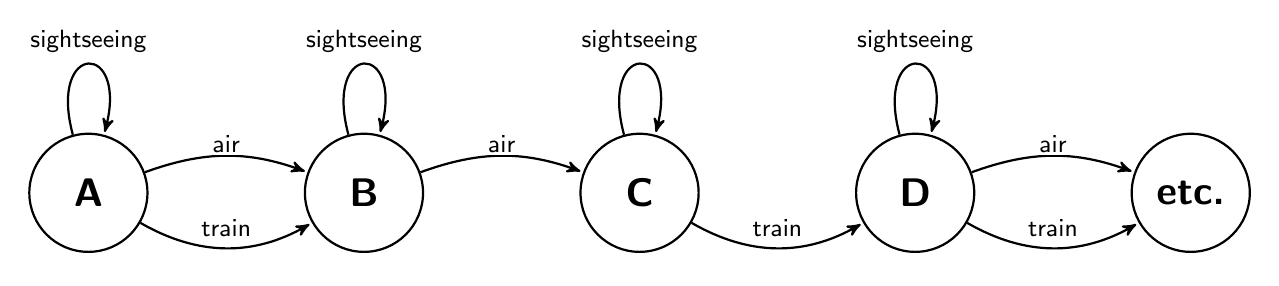
\begin{tikzpicture}[->,>=stealth',shorten >=1pt,auto,node distance=3.5cm,
  thick,main node/.style={circle,fill=white!20,draw,
  font=\sffamily\Large\bfseries,minimum size=15mm}]

  \node[main node] (A) {A};
  \node[main node] (B) [right of=A] {B};
  \node[main node] (C) [right of=B] {C};
  \node[main node] (D) [right of=C] {D};
  \node[main node] (E) [right of=D] {etc.};

  \path[every node/.style={font=\sffamily\small,
  		fill=white,inner sep=1pt}]
  	% Right-hand-side arrows rendered from top to bottom to
  	% achieve proper rendering of labels over arrows.
    (A) edge [loop above] node[above=1mm] {sightseeing} (A)
        edge [bend left=20] node {air} (B)
        edge [bend right=30]node[above=1mm] {train}(B)
    (B) edge [loop above] node[above=1mm] {sightseeing} (B)
        edge [bend left=20] node{air} (C)
    (C) edge [loop above] node[above=1mm] {sightseeing} (C)
        edge [bend right=30]node[above=1mm] {train}(D)
    (D) edge [loop above] node[above=1mm] {sightseeing} (D)
        edge [bend left=20] node{air} (E) 
        edge [bend right=30]node[above=1mm] {train}(E);
   
\end{tikzpicture}
\\